%; whizzy chapter
% -initex iniptex -latex platex -format platex -bibtex jbibtex -fmt fmt
% $B0J>e(B whizzytex $B$r;HMQ$9$k>l9g$N@_Dj!#(B

%     Kansai Debian Meeting resources
%     Copyright (C) 2007 Takaya Yamashita
%     Thank you for Tokyo Debian Meeting resources

%     This program is free software; you can redistribute it and/or modify
%     it under the terms of the GNU General Public License as published by
%     the Free Software Foundation; either version 2 of the License, or
%     (at your option) any later version.

%     This program is distributed in the hope that it will be useful,
%     but WITHOUT ANY WARRANTY; without even the implied warranty of
%     MERCHANTABILITY or FITNESS FOR A PARTICULAR PURPOSE.  See the
%     GNU General Public License for more details.

%     You should have received a copy of the GNU General Public License
%     along with this program; if not, write to the Free Software
%     Foundation, Inc., 51 Franklin St, Fifth Floor, Boston, MA  02110-1301 USA

%  preview (shell-command (concat "evince " (replace-regexp-in-string "tex$" "pdf"(buffer-file-name)) "&"))
% $B2hA|%U%!%$%k$r=hM}$9$k$?$a$K$O(Bebb$B$rMxMQ$7$F(Bboundingbox$B$r:n@.!#(B
%(shell-command "cd image200708; ebb *.png")

%%$B$3$3$+$i%X%C%@3+;O!#(B

\documentclass[mingoth,a4paper]{jsarticle}
\usepackage{kansaimonthlyreport}
\usepackage[dvips]{xy}
\usepackage{ulem}

% $BF|IU$rDj5A$9$k!"Kh7nJQ$o$j$^$9!#(B
\newcommand{\debmtgyear}{2014}
\newcommand{\debmtgdate}{25}
\newcommand{\debmtgmonth}{5}
\newcommand{\debmtgnumber}{84}

\def\fixme#1{{\color{red}{#1}}}

\begin{document}

\begin{titlepage}

% $BKh7nJQ99$9$kItJ,!"K\J8$NKvHx$b=$@5$9$k$3$H$r$o$9$l$:$K(B

 $BBh(B\debmtgnumber{}$B2s(B $B4X@>(B Debian $BJY6/2q;qNA(B

\vspace{2cm}

\begin{center}
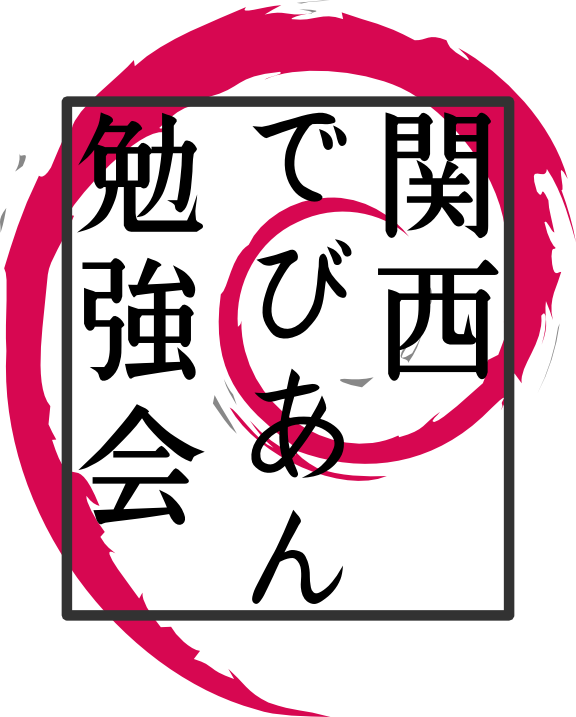
\includegraphics{image200802/kansaidebianlogo.png}
\end{center}

\begin{flushright}
\hfill{}$B4X@>(B Debian $BJY6/2qC4Ev<T(B $B:4!9LZ!&ARI_!&$N$,$?!&$+$o$@!&H,DEHx(B \\
\hfill{}\debmtgyear{}$BG/(B\debmtgmonth{}$B7n(B\debmtgdate{}$BF|(B
\end{flushright}

\thispagestyle{empty}
\end{titlepage}

\dancersection{Introduction}{Debian JP}

\vspace{1em}

 $B4X@>(BDebian$BJY6/2q$O(BDebian GNU/Linux$B$N$5$^$6$^$J%H%T%C%/(B
 ($B?7$7$$%Q%C%1!<%8!"(BDebian$BFCM-$N5!G=$N;EAH!"(BDebian$B3&7($G5/$3$C$?=PMh;v!"(B
 $B$J$I$J$I!K$K$D$$$FOC$79g$&2q$G$9!#(B

 $BL\E*$H$7$F<!$N;0$D$r9M$($F$$$^$9!#(B
 \begin{itemize}
  \item ML$B$d7G<(HD$G$O$J$/!"D>@\4i$r9g$o$;$k;v$G$N>pJs8r49$NB%?J(B
  \item $BDj4|E*$K=8$^$l$k>l=j(B
  \item $B;qNA$N:n@.(B
 \end{itemize}

 $B$=$l$G$O!"3Z$7$$0l;~$r$*2a$4$7$/$@$5$$!#(B

\newpage

\begin{minipage}[b]{0.2\hsize}
 {\rotatebox{90}{\fontsize{80}{80}
{\gt $B4X@>(B Debian $BJY6/2q(B}}}
\end{minipage}
\begin{minipage}[b]{0.8\hsize}
\hrule
\vspace{2mm}
\hrule
\setcounter{tocdepth}{1}
\tableofcontents
\vspace{2mm}
\hrule
\end{minipage}

\dancersection{$B:G6a$N(BDebian$B4X78$N%$%Y%s%HJs9p(B}{Debian JP}

\subsection{$BBh(B83$B2s4X@>(BDebian$BJY6/2q(B}

83$B2sL\$N4X@>(BDebian$BJY6/2q$O(B4$B7n(B27$BF|(B($BF|(B)$B$K!"J!Eg6hL1%;%s%?!<$G9T$J$o$l$^$7(B
$B$?!#(B

$B@n9>$5$s$K$h$k!V<+Bp%5!<%P$K(BKVM$B$rF3F~$7$F$_$h$&!W$H(BDavid Bremner$B$5$s$K(B
$B$h$k!V(BNotmuch Mail$B!W$NFsK\N)$F$G$7$?!#(B

$B$3$3$7$P$i$/9T$J$C$F$$$J$+$C$?%;%C%7%g%s7A<0!"$^$?3$30$+$i$N(BDebian
Developer$B$NMhK,$H$J$C$?JY6/2q$G$7$?!#(B

$BHs>o$K3Z$7$=$&$JFbMF$G$7$?$,;22C$G$-$J$+$C$?$N$,;DG0$G$9!#(B

\subsection{$BBh(B113$B2sEl5~%(%j%"(BDebian$BJY6/2q(B}

113$B2sL\$NEl5~%(%j%"(BDebian$BJY6/2q$O(B5$B7n(B17$BF|(B($BEZ(B)$B$K3t<02q<R%9%/%&%'%"!&%(%K%C(B
$B%/%9(B $B2q5D<<$G9T$J$o$l$^$7$?!#(B

$BLnEg$5$s$K$h$k!V(Bdebian $B$H(B docker.io$B!W$H$b$/$b$/$N2q$N7A<0$G9T$J$o$l$^$7(B
$B$?!#(B

Debian$B$G(Bdocker$B$r;H$C$F$_$F!"(BGoogle Compute Engine$B$G$bF0$+$7$F$_$h$&$H$$(B
$B$&FbMF$K$J$C$F$$$^$9!#N.9T$j$N(Bimmutable infrastructure$B$r(BDebian$B$G(Bdocker.io
$B$r;H$C$F;n$7$F$_$F$/$@$5$$!#(B

\subsection{Debian Project}

\subsubsection{Code of Conduct}

$B$3$3?t%v7n?($l$F$-$?$h$&$K!"(BDebian Project$B$O!"(BGR(General Resolution:$B0lHL7h5D(B)
$B$r$X$F(BCode of Conduct$B$,:NBr$5$l$^$7$?!#(B
$BEjI<7k2L$O!V0lHL7h5D(B: $BMxMQ>e$NCm0U!W(B
\footnote{\url{https://www.debian.org/vote/2014/vote_002}}
$B$K>\$7$$$G$9$,!"(BCode of Conduct$B$KBgB??t$,;?@.$@$C$?$b$N$N!"$=$N2~D{$r(B
DPL(Debian Project Leader)$B$,9T$J$&$+!"(BGR$B$rDL$7$F9T$J$&$+$O6O$+(B13$BI<:9(B
$B$G(BGR$B$rDL$7$F9T$J$&$3$H$K$J$j$^$7$?!#(B

systemd$B4XO"$N%U%l!<%`$,%a!<%j%s%0%j%9%H>e$G5/$3$C$?$3$H$KC<$rH/$7$F(B
Code of Conduct$B$r$H$NN.$l$K$J$j$^$7$?$,!":NBrD>8e$K$^$?(B200$B7o$r1[$($k(B
systemd$B4XO"$N%9%l%C%I$,(Bdebian-devel$B$K$?$C$F$$$?$j$7$^$9!#(B

\subsubsection{systemd/GNOME Sprint}

4$B7n(B25$BF|$+$i(B27$BF|$K$+$1$F!"%Y%k%.!<$N%"%s%H%o!<%W$G!V(Bsystemd/GNOME Sprint$B!W(B
\footnote{\url{https://wiki.debian.org/Sprints/2014/SystemdGNOMESprint}}
$B$,3+:E$5$l$^$7$?!#(B

$B!V(BBits from the systemd + GNOME sprint$B!W(B
\footnote{\url{https://lists.debian.org/debian-devel-announce/2014/05/msg00001.html}}
$B$NJs9p$K$h$k$H!"(Bsystemd$B4XO"$G$O(Budev$B$N@0M}!"(Bgit-buildpackage$B$NMxMQ$H%j%](B
$B%8%H%j$N@0M}!"%P!<%8%g%s(B208$B$N%Q%1!<%8%s%0!"(BGNOME$B4XO"$G$O!"3F%Q%C%1!<%8(B
$B$N0\9T!"(BVCS$B$N(BSubversion$B$+$i(Bgit$B$X$N0\9T$N8!F$!"(Bjessie$B$G$N(BGNOME 3.14$B$N2D(B
$BG=@-!"(BBluez5$B$X$N<h$jAH$_!"$J$I$J$I$,9T$J$o$l$^$7$?!#(B

systemd$B$H(BGNOME$B$H$$$($PI.<T$O:G6a!"(B
\debianbug{747210}$B!V(Bgdm3: fails to restart X server after first logout, screen blank$B!W(B
$B$KAx6x$7$?$N$G(Binit$B$r(Bsystemd$B$KJQ99$7$F2sHr$7$?$i!"(B
\debianbug{746358}$B!V(Bsystemd: system boot hangs if /etc/fstab contains an NFS mount$B!W(B
$B$KAx6x$9$k$H$$$&%3%s%\$K%O%a$i$l$^$7$?!#(B

\subsubsection{$B%j%j!<%9$K8~$1$F(B}
$B!V(BBits from the Release Team - Freeze, removals and archs$B!W(B
\footnote{\url{https://lists.debian.org/debian-devel-announce/2014/05/msg00000.html}}
$B$G%j%j!<%9%A!<%`$+$i(B6$B%v7n$r@Z$C$?(Bjessie$B$N%U%j!<%:$^$G$N%?%$%`%F!<%V%k(B
$B$,Js9p$5$l$^$7$?!#$^$?3F%"!<%-%F%/%A%c$N>uBV$b$"$o$;$FJs9p$5$l$F$$$^$9!#(B

$BCf$G$b(BHurd$B$K$D$$$F$O!V(BBits from the Debian GNU/Hurd porters$B!W(B
\footnote{\url{https://lists.debian.org/debian-devel-announce/2014/05/msg00006.html}}
$B$G!"(BDebian GNU/Hurd$B$G(BDebian$B$NLs(B8$B3d$N%Q%C%1!<%8$r;HMQ$G$-$k$3$H(B(Iceweasel
$B$b(B29$B$G(BSSL$B$,;H$($^$9(B)$B!"(Binit$B%7%9%F%`$r(BSysVinit$B$KJQ99$7$?$3$H!"(Bpthread$B$K$J$C(B
$B$?$3$H!"%M%C%H%o!<%/%I%i%$%P$,(BDDE(Device Driver Environment)$B%U%l!<%`%o!<(B
$B%/%Y!<%9$K$J$C$?$3$H!"$J$I$J$I$,Js9p$5$l$F$$$^$9!#(B

$BJs9p$K$O5s$,$C$F$$$J$$%"!<%-%F%/%A%c$G$9$,!"(Barm64$B$H(Bmips64el$B$b3hH/$K3+H/(B
$B$,?J$s$G$$$k$h$&$G$9!#(B
arm64$B$K$D$$$F$O(B
$B!V(BArm64 port live on debian-ports$B!W(B
\footnote{\url{https://lists.debian.org/debian-devel/2014/04/msg00509.html}}
$B$H!V(Barm64 update - help wanted$B!W(B
\footnote{\url{https://lists.debian.org/debian-devel/2014/05/msg00666.html}}
$B$K$h$k$H!"(B2$B$D$N(Bbuildd$B$rAv$i$;$F$*$j!"(B4200$B$N%=!<%9%Q%C%1!<%8$,%S%k%I$G$-(B
$B$F$$$^$9!#(B
mips64el$B$K$D$$$F$O(B
$B!V(Bmips64el: FTBFS list and buildlogs$B!W(B\footnote{\url{https://lists.debian.org/debian-devel/2014/04/msg00809.html}}
$B$K$h$k$H!"(B7000$B0J>e$N%Q%C%1!<%8$N%S%k%I$K@.8y$7$F$*$j!"(B1000$B0J>e$,%S%k%I(B
$BBT$A$H$J$C$F$$$^$9!#(B

\subsubsection{CTTE}
$B!V(BMaximum term for tech ctte members$B!W(B
\footnote{\url{https://lists.debian.org/debian-project/2014/05/msg00054.html}}
$B$G(BCTTE$B$N%a%s%P!<$KG$4|$r@_$1$F$O$I$&$+$H$$$&5DBj$,$"$,$C$F$$$^$9!#(B

CTTE$B$H$O(BDebian Technical Committee\footnote{\url{https://www.debian.org/devel/tech-ctte}}
$B$H$$$&(BDebian$B%W%m%8%'%/%HFb$N5;=QE*$JO@Ah$K:G=*E*$J7hCG$r2<$9=8CD$G$9!#(B
$B:G6a$G$O(BJessie$B$N(BLinux$B%"!<%-%F%/%A%c$G$N%G%U%)%k%H(Binit$B%7%9%F%`$r(Bsystemd
$B$K$9$k$Y$-$H$N7hDj$r$7$F$$$^$9!#(B

$BG$4|$r2?G/$K$9$k$+!"8=9T@)EY$+$i$I$N$h$&$K0\9T$9$k$+!"$^$@5DO@$O$O$8$^$C(B
$B$?$P$+$j$G$9$,!"35$M;?F1$9$k0U8+$,B?$$$h$&$G$9!#(B
$B$A$J$_$K!"8=%a%s%P!<$G$N:G8E;2$O(BIan Jackson$B$5$s$G(B15$BG/(B5$B%v7nL\$K$J$j$^$9!#(B

\subsubsection{debian-devel}
\begin{itemize}
\item $B!V(BCall for help from KDE Team$B!W(B\footnote{\url{https://lists.debian.org/debian-devel/2014/05/msg00008.html}}\\
  KDE$B%A!<%`$+$i$N%X%k%WMW@A!#(B

\item $B!V(BGhostscript licensing changed to AGPL$B!W(B\footnote{\url{https://lists.debian.org/debian-devel/2014/05/msg00144.html}}\\
  Ghostscript$B$N%i%$%;%s%9$,(BAGPL$B$KJQ$C$F$$$?$N$G4XO"%Q%C%1!<%8$K1F6A$,$"(B
  $B$k$N$G$O$J$$$+!#(B

\item $B!V(BRemoval of emacs23 from unstable/testing$B!W(B\footnote{\url{https://lists.debian.org/debian-devel/2014/05/msg00167.html}}\\
  Jessie$B%U%j!<%:A0$K(Bemacs23$B$r=|5n$7$?$$!#(B

\item $B!V(Bsystemd-fsck?$B!W(B\footnote{\url{https://lists.debian.org/debian-devel/2014/05/msg00255.html}}\\
  systemd$B$OA4$F$r>h$C<h$k5$$+!)$+$i;O$^$C$?(B200$B7o$r1[$($k%9%l%C%I!#FI$s$G$J$$!#(B

\item $B!V(BMedia type vnd.debian.binary-package accepted by the IANA.$B!W(B\footnote{\url{https://lists.debian.org/debian-devel/2014/05/msg00792.html}}\\
  $B%a%G%#%"%?%$%W$K(BDebian$B$N%P%$%J%j%Q%C%1!<%8$G$"$k(B.deb$B$H(B.udeb$B$,EPO?$5$l$?!#(B

\item $B!V(BBug\#747596: ITP: liblxqt-mount -- Library used to manage removable devices for LXDE-Qt$B!W(B\footnote{\url{https://lists.debian.org/debian-devel/2014/05/msg00314.html}}\\
  $B!V(BBug\#747597: ITP: lxqt-config -- LXQt system settings center$B!W(B\footnote{\url{https://lists.debian.org/debian-devel/2014/05/msg00315.html}}\\
  $B!V(BBug\#747598: ITP: lxqt-config-randr -- Qt config GUI for X11 RandR for LXQt system settings$B!W(B\footnote{\url{https://lists.debian.org/debian-devel/2014/05/msg00316.html}}\\
  $B!V(BBug\#747599: ITP: lxqt-common -- Common files for LXQt$B!W(B\footnote{\url{https://lists.debian.org/debian-devel/2014/05/msg00317.html}}\\
  $B!V(BBug\#747600: ITP: lxqt-about -- The standalone LXQt "About" dialog$B!W(B\footnote{\url{https://lists.debian.org/debian-devel/2014/05/msg00318.html}}\\
  $B!V(BBug\#747601: ITP: lxqt-globalkeys -- Daemon used to register global keyboard shortcuts$B!W(B\footnote{\url{https://lists.debian.org/debian-devel/2014/05/msg00319.html}}\\
  $B!V(BBug\#747602: ITP: lxqt-notificationd -- The LXQt notification daemon$B!W(B\footnote{\url{https://lists.debian.org/debian-devel/2014/05/msg00320.html}}\\
  $B!V(BBug\#747603: ITP: lxqt-openssh-askpass -- OpenSSH user/password GUI dialog for LXQt$B!W(B\footnote{\url{https://lists.debian.org/debian-devel/2014/05/msg00321.html}}\\
  $B!V(BBug\#747604: ITP: lxqt-qtplugin -- LXDE-Qt platform integration plugin for Qt$B!W(B\footnote{\url{https://lists.debian.org/debian-devel/2014/05/msg00322.html}}\\
  $B!V(BBug\#747605: ITP: pcmanfm-qt -- File manager and desktop icon manager (Qt port of PCManFM and libfm)$B!W(B\footnote{\url{https://lists.debian.org/debian-devel/2014/05/msg00323.html}}\\
  $B!V(BBug\#747607: ITP: lxqt-policykit -- The LXQt PolicyKit agent$B!W(B\footnote{\url{https://lists.debian.org/debian-devel/2014/05/msg00324.html}}\\
  $B!V(BBug\#747608: ITP: lxqt-session -- An alternative session manager ported from the original razor-session$B!W(B\footnote{\url{https://lists.debian.org/debian-devel/2014/05/msg00325.html}}\\
  $B!V(BBug\#747610: ITP: lxqt-panel -- The LXQt desktop panel$B!W(B\footnote{\url{https://lists.debian.org/debian-devel/2014/05/msg00326.html}}\\
  $B!V(BBug\#747611: ITP: lxqt-powermanagement -- Power management module for LXQt$B!W(B\footnote{\url{https://lists.debian.org/debian-devel/2014/05/msg00327.html}}\\
  $B!V(BBug\#747613: ITP: lxqt-runner -- Tool used to launch programs quickly by typing their names$B!W(B\footnote{\url{https://lists.debian.org/debian-devel/2014/05/msg00328.html}}\\
  $B!V(BBug\#747620: ITP: liblxqt -- Core utility library for all LXDE-Qt components$B!W(B\footnote{\url{https://lists.debian.org/debian-devel/2014/05/msg00332.html}}\\
  Andrew Lee$B$K$h$k(BLXDE-Qt$B4XO"%Q%C%1!<%8$NE\Es$N(BITP$B!#(B

\end{itemize}

\dancersection{$B;vA02]Bj(B}{Debian JP}

$B:#2s$N2]Bj$O0J2<$NDL$j$G$9!#(B
\begin{screen}
  \begin{enumerate}

  \item %
    $B$b$/$b$/$N2q$G9T$J$&:n6H!"<ALd$J$I$N2]Bj$rMQ0U$7$F65$($F$/$@$5$$!#(B
    ($BEE8;$H%M%C%H%o!<%/(B(WiMAX$B$J$I(B)$B$O$"$j$^$9$,!"$=$l0J30$N:n6H$KI,MW$J(B
    $B4D6-$O$4MQ0U$/$@$5$$!#(B)

  \item %
    $BA02s(B($BBh(B83$B2s(B)$B$NJY6/2q$K;22C$5$l$?J}$O!"A02s$N:n6H$d2]Bj$,$=$N8e$I$&(B
    $B$J$C$?$+7k2L$r65$($F$/$@$5$$!#(B

  \item %
    LT($B%i%$%H%K%s%0%H!<%/(B) $B4?7^$G$9!#2?$+$*OC$7$?$$J}$O%?%$%H%k$r2<$5$$!#(B
  \end{enumerate}
\end{screen}

$B;22C<T$N3'$5$s$N2rEz$O0J2<$NDL$j$G$9(B:

\begin{prework}{ $B$+$o$@$F$D$?$m$&(B }
  \begin{enumerate}
  \item $B2?$+MQ0U$7$F$*$-$^$9!#(B
  \item $B;22C$G$-$^$;$s$G$7$?!#(BNotmuch Mail...
  \item $B$$$D$b$N(BDebian Project$B$NOCBj$r>R2p$7$^$9!#(B
  \end{enumerate}
\end{prework}

\begin{prework}{ murase\_{}syuka }
  \begin{enumerate}
  \item mruby$B%Q%C%1!<%899?7(B
  \item $BIT;22C(B
  \item $BFC$KL5$7(B
  \end{enumerate}
\end{prework}

\begin{prework}{ takata }
  \begin{enumerate}
  \item $B$$$D$b<ALd$P$+$j$G$9$_$^$;$s!#(B

    Wake on LAN$B$G(B PC$B$r5/F0$9$k>l9g!"0E9f2=(BLUKS$B%Q!<%F%#%7%g%s$N%Q%9%o!<%I$r0BA4$KF~NO$9$k$K$O$I$&$9$k$N$,$h$$$G$7$g$&!)(B

    $B%^%8%C%/%Q%1%C%H$r;H$C$?(B Wake on LAN$B$G$O!"%Q%9%o!<%I$r%Z%$%m!<%I$H$7$FEj$2$k$h$&$J5!G=$O$J$$$h$&$K$_$($^$9!#(B

    $B$"$i$+$8$a0J2<$N$h$&$JJ}K!$G(B LUKS$B%Q%9%o!<%I$NF~NO$r>JN,$9$k$h$&$K@_Dj$7$F$*$-!"(BWake on LAN$B$G$O%^%8%C%/%Q%1%C%H$rEj$2$D$1$FEE8;(BON$B$K$9$k$@$1$K$9$k!"$H$+$G$7$g$&$+!#(B

    \url{http://www.howtoforge.com/automatically-unlock-luks-encrypted-drives-with-a-keyfile}
  \end{enumerate}
\end{prework}

\begin{prework}{ $B:4!9LZMNJ?(B }
  $B;22C$7$^$9!#(B

  ruby $B4XO"$N0\9T$,%a%$%s!"$+$J!#(B
\end{prework}

\begin{prework}{ $B@n9>(B }
  \begin{enumerate}
  \item $B$H$j$"$($:!"(BHTML5$B$G$N%5%$%H$N:n@.$H!"<+Bp%5!<%P$N@0Hw!#(B
  \item $BF1>e(B
  \end{enumerate}
\end{prework}

\begin{prework}{ lurdan }
  \begin{enumerate}
  \item $B$$$/$D$+(B BTS $B$?$^$C$F$-$F$k$N$G$=$l$rJR$9!"$b$7$/$O(B webwml-git $B$N7o$r$b$&$A$g$C$H(B
  \end{enumerate}

  $B=jMQ$N$?$aESCf$GH4$1$^$9(B
\end{prework}

\begin{prework}{ yyatsuo }
\end{prework}

\begin{prework}{ Hiroyuki Nagata }
  \begin{enumerate}
  \item D$B8@8l$r$J$s$+=q$/$+(Bo2on$B$N%]!<%F%#%s%0:n6H(B
  \item JaneClone$B$r(BITP$B$7$^$7$?(B
  \item $B$H$/$K$J$7$G$9(B
  \end{enumerate}
\end{prework}

\dancersection{$B$b$/$b$/$N2q(B}{}

\dancersection{$B:#8e$NM=Dj(B}{Debian JP}

\subsection{$B4X@>(BDebian$BJY6/2q(B}

$B<!2s!"Bh(B85$B2s4X@>(BDebian$BJY6/2q$O(B6$B7n(B22$BF|(B($BF|(B)$B$KJ!Eg6hL1%;%s%?!<$G3+:E$7$^$9!#(B

$B$^$?!":#G/$b(B8$B7n$K3+:E$5$l$k(BOSC 2014 Kansai@Kyoto$B$K=PD%3+:EM=Dj$G$9!#(B
$B:#G/$O?7$7$$(BT$B%7%c%D$,$"$k$+$b$7$l$^$;$s!#(B

\subsection{$BEl5~%(%j%"(BDebian$BJY6/2q(B}
$BBh(B114$B2sEl5~%(%j%"(BDebian$BJY6/2q$O(B6$B7n(B14$BF|(B($BEZ(B)$B$K3t<02q<R%9%/%&%'%"!&%(%K%C(B
$B%/%9(B $B%;%_%J!<%k!<%`$G3+:EM=Dj$G$9!#(B
$B3+:EF|$,$$$D$b$NBh;0EZMKF|$G$O$J$/!"BhFsEZMKF|$H$J$C$F$$$^$9$N$G$4Cm0U(B
$B$/$@$5$$!#(B

$BFbMF$O!"(Bwbcchsyn$B$5$s$K$h$k!V(BGPG $BHkL)80<h$j07$$J}K!$NDs0F!W$H$$$&!"(BGPG$B$N(B
$BHkL)804IM}$K$D$$$F$N%"%$%G%"$r8l$k$H$J$C$F$$$^$9!#(B

%
% $B:};R$K$9$k$?$a$K!"(B4$B$NG\?t$K$9$kI,MW$,$"$k!#(B
% $B$=$N$?$a$ND4@0(B
\dancersection{$B%a%b(B}{}
\mbox{}\newpage
%% \mbox{}\newpage
%% \mbox{}\newpage

\printindex
%\cleartooddpage

 \begin{minipage}[b]{0.2\hsize}
  \rotatebox{90}{\fontsize{80}{80} {\gt $B4X@>(B Debian $BJY6/2q(B} }
 \end{minipage}
 \begin{minipage}[b]{0.8\hsize}

 \vspace*{15cm}
 \rule{\hsize}{1mm}
 \vspace{2mm}
 
\includegraphics[width=2cm]{image200502/openlogo-nd.eps}
 \noindent \Large \bfseries{Debian $BJY6/2q;qNA(B}\\ \\
 \noindent \normalfont \debmtgyear{}$BG/(B\debmtgmonth{}$B7n(B\debmtgdate{}$BF|(B \hspace{5mm}  $B=iHGBh(B1$B:~H/9T(B\\
 \noindent \normalfont $B4X@>(B Debian $BJY6/2q(B $B!JJT=8!&0u:~!&H/9T!K(B\\
 \rule{\hsize}{1mm}
 \end{minipage}

\end{document}
